\documentclass[a4full,12pt]{article}

\title{Integrating a Category-Partition Testing Tool with Combinatorial Interaction
Testing Tool To Produce T-Way Adequate Test Frames}
\author{Andrew Graff}

%\usepackage{fullpage}
%\usepackage{epsfig}
\usepackage{graphicx}
\usepackage{xcolor}
\graphicspath{ {./images/} }

\newcommand{\eas}[1]{{\color{blue}\sf ({#1})}}
\newcommand{\ag}[1]{{\color{red}\sf ({#1})}}
\renewcommand{\topfraction}{.9}
\renewcommand{\bottomfraction}{.9}
\renewcommand{\textfraction}{.1}
\begin{document}
\maketitle
\section{Introduction}
Software is the beating heart of a lot of technology today, and defects in that software
  can be costly. Some simply print funny characters to the terminal, while some can bring
  your production to a halt for hours or even days costing thousands and even millions of
  dollars. Or perhaps a security breach which exposes your intellectual property which
  could kill your business altogether. That is why testing is such an important step in
  the process of creating defect free software. Testing software can be a difficult task
  depending on the complexity of the software itself, what kind of inputs it takes, and how
  many different functions it can perform. And there are several different approaches in how
  to do the actual testing: black-box, white-box, static analysis to name a few. We will be
  focusing on black-box testing, and more specifically generating test cases that find the
  greatest amount of defects with a realistically executable number of test cases.
  
\section{Problem Statement and Proposed Solution}
  \eas{Here you can state the main point of what you are proposing -- combining TSL (testing specification language), i.e., the front-end of the category partitioning method with combinatorial interaction testing, which has no useful front-end}
It is difficult to engineer a set of tests that adequately tests a particular piece of software
  in an acceptable amount of time. Category partitioning is a useful black-box testing method that
  helps to test systematic design with test cases. It allows the user to divide
  the inputs of the software into categories of choices. TSL (testing specification language) is a tool
  that offers a good front-end for the category partitioning method with a formal descriptive language
  to specify how the program works using categories and choices. In addition, TSL will generate tests
  cases in an output file. However, it's weakness is that it will generate all possible permutations of
  the categories and choices as test frames, which may not run in a feasible amount of time.
  
Combinatorial interaction testing addresses the problem of the brute force approach of running all
  possible inputs by offering a method for analyzing and selecting a subset of test cases. The tool
  we will use for this step will be 


\eas{Here you can start that combinatorial interaction testing addresses this problem by finding test cases where only certain category choices appear together}
 Similarly, combinatorial interaction testing is useful for defining a subset of tests that satisfy a t-way pairwise interaction using a model and constraints file. \eas{Give three to four more sentence about how  CASA tool does it}\eas{ Then talk about its front end -- in fact its front-end is quite confusing that might introduce errors especially when expressing constraints. You might also state that in general an industry tester would not be able to use such tool --- how many would be able to express a constraint in a conjunctive normal form? Or decode the resulting output file.}
 
\eas{Here you should talk how you propose to solve this problem. The goal of this project is to ...} These two methodologies and tools\eas{you never mentioned any tools -- mention them in their corresponding paragraphs} are separate pieces of software that require the user  to generate the input to both tools. This project takes on the task of combining\eas{the user-friendly input/output components of one and integrate them into powerful test selection algorithm of another} these two powerful methods and tools so that the user only needs to generate the category partition test specification, and an adequate coverage set of test frames is generated eliminating the need for the engineer to create the model or constraints for the combinatorial interaction testing.

  
\section{Background}
\eas{Have  a better transition, e.g., This section presents background information on both methodologies and their corresponding tools. In particular, ...}
This project builds on the work of two teams that have come up with solutions to
  two different problems. Here we will explain each of those solutions and the 
  tools created to support them.

The \emph{category-partition method} uses a formal test specification language to generate
  test case descriptions. These test case descriptions would then be used to
  create an executable software test. So how do you generate the formal test 
  specifications? Depending on the size of the software system to test, the 
  engineer may need to break the program up into smaller testable blocks. For 
  the purposes of this project, we will use a simple example of a browser's 
  settings for how to treat tabs.
\begin{figure}[htb]
\centering
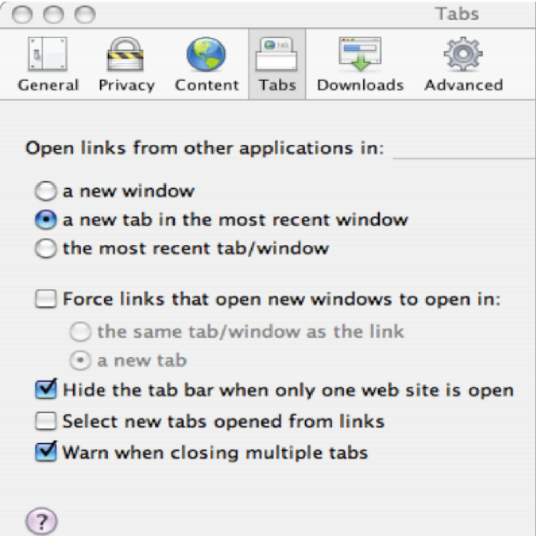
\includegraphics[width=2.3in,keepaspectratio]{images/tabs_example.png}
\caption{Sample of software feature to test tabs}
\label{fig:tabs_example}
\end{figure}

As part of the process to translate this feature into the formal language of \emph{tsl},
  we need to follow a specific format for our test specification file. It specifies
  \emph{categories}, \emph{choices}, \emph{properties}, and \emph{selectors} where 
  \emph{selectors} are boolean expressions. The format of the file looks like this:
\begin{figure}[htb]
\centering
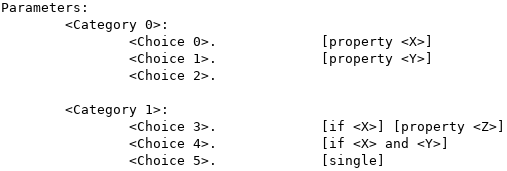
\includegraphics[width=3in,keepaspectratio]{images/tsl_format.png}
\caption{Format for tsl input file}
\label{fig:tsl_format}
\end{figure}

Back to our example, we need to choose \emph{categories} and \emph{choices} within those
  \emph{categories}. For example, one \emph{category} could be 'Link', and the choices
  associated with 'Link' are 'new window', 'new tab', and 'current tab' pulled from the
  'Open links from other applications in:' portion of the settings. We do this for all
  the available selections in this browsers 'Tabs' options and end up with the this for
  and input to \emph{tsl}
\begin{figure}[htb]
\centering
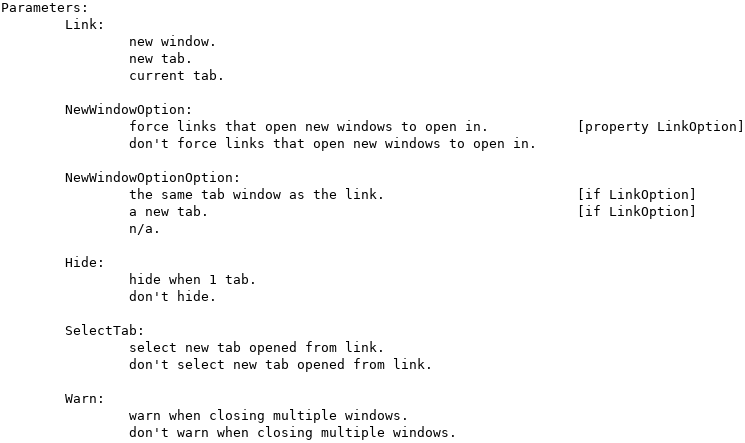
\includegraphics[width=4in,keepaspectratio]{images/tsl_input_final.png}
\caption{Example of first category of tabs example}
\label{fig:tsl_input_final}
\end{figure}

After executing \emph{tsl} for this simple example, we end up with 96 total test frames
  for all possible combinations of our \emph{categories} and \emph{choices}. This is a
  small example with very few choices. You can imagine an airplane cockpit with many
  switches and inputs. How many possible combinations would there be to test that? We
  need a way to reduce this test set down to a reasonably testable number.
  
  
The \emph{tsl} tool consists of 12 files and 1125 lines of code.
\ag{Still building on this. I've inserted the tsl portion above. 2/26/2021}
\ag{I will get the details of this program, loc, etc. 3/19/2021}
\eas{I have not given much of feedback here since it does need substantial information on
  \begin{itemize}
  \item The idea of black-box testing -- test selection based on the input space of a program
  \item Partition of the input space into equivalent classes
  \item Category partition method as a systematic way multi-level way of partition the input space
  \item TSL as a formal language to express those categories and paritions
  \item Existence of constraints between choices of different categories
  \item Resulting frames
  \item Refinement and coarsening of the spcification
  \item The tool description - lines of code and such
  \end{itemize}
  %Also the example on Figure~\ref{fig:tsl_input} is too large - try create something smaller, similar what we use in class -- new link in a browser setting
}


\emph{Combinatorial interaction testing} is a testing method that relies on the principle
  that a large portion of faults can be detected with a subset of the total number of 
  possible inputs. \emph{casa} is a tool that will find a \emph{t-way} pairwise covering 
  array that satisfies all possible values for each input within it's pair in order to find
  the minimal set of inputs to cover those faults using \emph{combinatorial interaction
  testing}. The tool takes two files as input: one that specifies the \emph{t-way} interaction
  level desired along with all possible inputs and one that describes constraints on those
  inputs. The output is the subset of combinations that satisfy the selected \emph{t-way}
  interaction level. This allows us to identify the subset of tests necessary to get adequate
  testing coverage. The inputs must be manually generated by the user and the connstraints
  file uses conjunctive normal form, which can be difficult to translate from prepositional
  logic we typically think and program in. In addition, the output may need some manual
  manipulation to translate back to something useful for testing.
  
The \emph{.citmodel} input file has the following format. The first line of the file
  specifies the strength of the T-way pairs to find. The second line specifies the number
  of \emph{categories} we have broken the program into. And the third line specifies how
  many \emph{choices} within the categories we have start from the first \emph{category} to
  the last. \ref{fig:casa_citmodel_input}
The \emph{casa} tool consists of 87 files with 9139 lines of code.
  
\begin{figure}[htb]
\centering
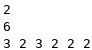
\includegraphics[width=1in,keepaspectratio]{images/casa_citmodel_input.png}
\caption{Example of CASA .citmodel input file}
\label{fig:casa_citmodel_input}
\end{figure}

\ag{Added the above. Still working on covering the list below. I will fill in more details this weekend. 3/19/2021} 
\eas{Make sure you address the following
\begin{itemize}
\item The premise of t-way testing (defects occurs when few choices of categories interact, e.g., two choices)
\item An overall approach of CIT test case selection.
\item CASA tool and its input and output format examples, emphasize that it is not user-friendly. Moreover, a compound constraint among choices should be converted into a conjunctive normal form (CNF), i.e., "AND" of "ORs" between choices
\item Have some metric of this tool - lines of code and such
\end{itemize}
}

%\begin{figure}[htb]
%\centering
%\includegraphics[width=4in,keepaspectratio]{images/casa_constraints_input.png}
%\caption{Example of first category of tabs example}
%\label{fig:casa_constraints_input}
%\end{figure}

\begin{figure}[htb]
\centering
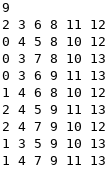
\includegraphics[width=4in,keepaspectratio]{images/casa_output.png}
\caption{Example of first category of tabs example}
\label{fig:casa_output}
\end{figure}

\section{Preliminary Work}
Some preliminary work has been done on this project in order to determine the
  feasibility of the idea to combine the \emph{tsl} and \emph{casa} tools into 
  a single, easy to use tool. A goal of the project is to simplify and reduce the
  effort a user needs to put in to use the new tool. Source code was acquired for
  both tools and some initial analysis of the code was done in order to understand
  how they work and where some work may be needed to combine them. As it
  turns out, the \emph{tsl} tool is written in basic C and \emph{casa} is written
  in C++. Converting \emph{tsl} to C++ would be beneficial for combining the 
  code bases into a single program. So \emph{tsl} was updated to support compilation
  with the g++ compiler.

As part of the simplification of the tool, only the category partition test specifications
  should need to be created by the user as a \emph{.tsl} file. The tool will do the rest to
  generate the adequate coverage set of test frames. Since \emph{casa} takes as input a 
  \emph{.citmodel} file, this preliminary version of \emph{tsl} generates one based on the
  specification file passed in. The generation of the \emph{.constraints} file will be created
  at a later time as part of the proposed work. In order to create the \emph{.citmodel}, we need
  to be able to keep track of the parsed information from the specifications file.
  
\ag{I'm still working on the portion below 2/26/2021}    
\eas{I think below you have all the information written well. However it would be better if instead of starting a paragraph
  talking about \em{what you've done} and then \em{why you did it}, you switch the order. State first what needs to be done:
  (1) establishing the map between categories and their choices and casa input values;
  (2) invoking casa on the translated input;
  (3) interpreting casa's output to produce frames}
  
In order to achieve this, a new struct was added to \emph{tsl/structs.h} called \emph{container} that
  keeps track of the list of non-single Choices as a vector of Choice struct
  pointers.\eas{Make sure you explain in your background section what is Choice - by the way why is it capitalized?} This vector is used to lookup the choices and categories later for
  printing the test frames. In addition, a \emph{parent} pointer was added to
  the Choice struct so that the Category information can be referenced when
  performing the lookup into the Choice* vector.
  
Rather than output directly all possible test frames, a new function called
  \emph{make\_citmodel()} was written in \emph{tsl/output.c} to write a 
  \emph{.citmodel} file used as an input to \emph{casa}. The function
  \emph{generator(Flag flags)} was also modified to call \emph{make\_citmodel()},
  and then make a system call to casa passing in the \emph{.citmodel} file for
  the input. Then, another function created  called
  \emph{process\_output\_file(string filename)} processes the file output by
  \emph{casa} to generate the test frame final output. Ideally there should be
  no file io required, but this is a preliminary draft of the final solution
  and will be addressed in the final version of the project.
  
  \section{Proposed Remaining Work}
Arguably the bulk of the work will be to translate the \emph{properties} and 
  \emph{contraints} defined in the category partition test specifications into
  the constraints file required by \emph{casa} to properly generate the adequate
  set of test frames rather than all possible combinations. \eas{Maybe one of those days we can talk about how we can outline this approach in general}
  
  https://github.com/Panik-Kontrol/MastersProject

\end{document}
